\section{Proxy}


Das Proxy Design Pattern lässt den Client einer Komponente mit einer Repräsentation anstatt der Komponente selbst kommunizieren. Einen soclhen Platzhalter einzufügen kann verschiedenen Gründen dienen, wie einer erbesserten Effizienz, einfacherem Zugriff oder schutz vor unauthorisiertem Zugriff.

\subsection*{Example}


Die Miterarbeiter der Entwicklungsabteilung einer Firma rufen regelmässig Datenbanken ab für Informationen über Materialzulieferer, verfügbaren Teilen, technischen Zeichnungen und so weiter. Jeder entfernte Zugriff kann kostspielig sein, während viele dieser Zugriffe ähnliche oder identische Informationen abrufen und regelmässig passieren. Diese Sitaution lässt klar Raum für Verbesserungen bei den Zugriffszeiten und -kosten. Jedoch wollen wir nicht den Code der Entwicklerapplikationen mit solchen Optimierungen belasten. Die Anwesenheit und die Art einer Optimierung soll möglichst Transparent dem Benutzer und dem Programmierer gegenüber sein.

\subsection*{Context}


Ein Client benötigt Zugriff auf die Dienste einer anderer Komponente. Direkter Zugriff ist technisch möglich, aber möglicherweise nicht der beste Ansatz.

\subsection*{Problem}


Es ist oft unangemessen auf Komponenten direkt zuzugreifen.

\subsubsection*{Forces}

\begin{itemize}
	\item Der Zugriff auf die Komponente soll Laufzeit-Effizient, Kosten-Effizient und sicher sowohl für den Client als auch für die Komponente sein.
	\item Der Zugriff auf die Komponente soll transparent und einfach für die Client sein. Der Client soll insbesondere kein anderes Verhalten oder eine andere Syntax verwenden müssen, als das wenn er eine Komponente direkt aufruft.
	\item Der Client sollte sich bewusst über mölcihte Performance- oder Finanz-Einbussen sein beim Aufruf von Remote-Clients. Volle Transparenz kann die Kostendifferenz zwischen Diensten verschleiern.
\end{itemize}

\subsection*{Solution}


Lass den Client mit einer Repräsentation anstatt der Komponente selbst kommunizieren. Diese Repräsentation - Proxy genannt - bietet die Schnittstelle (Interface) der Komponente an aber führt zusätliche Pre- und Postbearbeitung durch, wie Zugriffskontrollen oder das Erstellen von Read-Only-Kopien des Originals.

\subsection*{Structure}
% Das ist ein forwarder receiver. wtf.
%\begin{figure}[H]
%	\centering
%	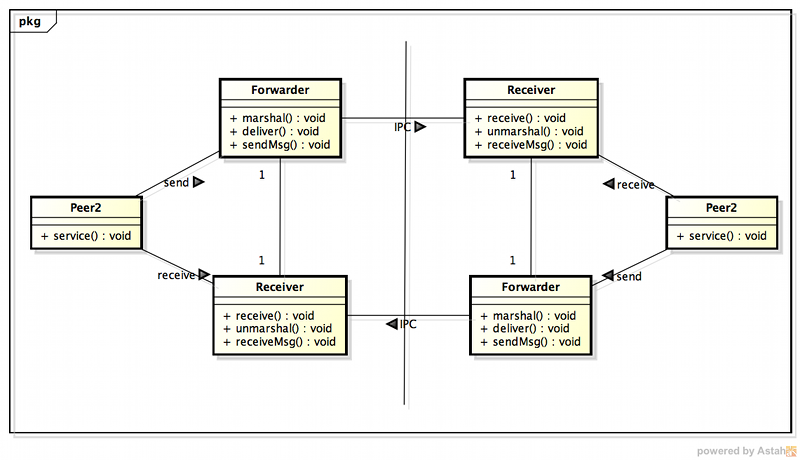
\includegraphics[width=0.7\textwidth]{content/posa1/images/proxy-classes.png}
%	\caption{Proxy Klassendiagramm}
%\end{figure}

Der Client ist verantwortlich für eine bestimmte Aufgabe. Um diese zu erledigen führt er die Funktionalität des Originals indirekt auf, indem er einen Proxy benutzt.

Dazu muss der Proxy die selbe Schnittstelle bereitstellen wie das Original und den korrekten Zugriff auf das Original sicherstellen. Dazu hält der Proxy eine Referenz auf das Original dass er repräsentiert. Normalerweise gibt es eine eins zu eins Beziehungs zwischen Proxy und Original. Allerdings gibt es Ausnahmen zu dieser Rgel für Remote und Firewall Proxies, zwei Varianten dieses Patterns.

Das "Abstract Original" liefert die vom Proxy und Original implementierte Schnittstelle.

\subsection*{Dynamics}

% Das ist ein forwarder receiver
%\begin{figure}[H]
%	\centering
%	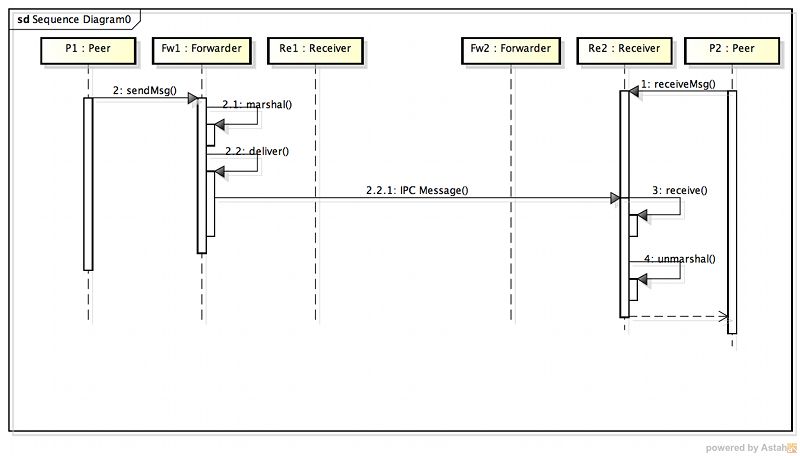
\includegraphics[width=0.7\textwidth]{content/posa1/images/proxy-sequence.png}
%	\caption{Proxy Sequenzdiagramm}
%\end{figure}

\begin{enumerate}
	\item png
	\item Für das Bewältigen einer Aufgabe bittet Client den Proxy einen bestimmten Dienstauzuführen.
	\item Der Proxy empfängt die eingehenden Dienst-Anfrage und führt ein Pre-Processing durch. Dieses Pre-Processing kann zum Beispiel das Auffinden der Adresse des Originals oder das Überprüfen eines lokalen Caches auf die Antwort der Anfrage sein.
	\item Falls der Proxy das Original benögit um die Anfrage auszuführen, leitet es den Request an das Original weiter.
	\item Das Original akzeptiert die Anfrage und führt sie aus. Es sendet die Antwort zurück an den Proxy.
	\item Der Proxy empfängt die Antwort. Vor oder nach dem Übermittel der Antwort an den Client führt der Proxy noch ein Post-Processing durch, wie zum Beispiel das Hinzufügen der Antwort zum lokalen Cache, den Destruktor des Originals aufrufen oder einen Lock auf eine Resource freigaben.
\end{enumerate}


\begin{enumerate}
	\item Identifiziere alle Verantwortlichkeiten für die Zugrisskontrolle (Access Control) einer Komponente. Weise diese Verantwortlichkeiten einer eigenen Komponente zu, dem Proxy.
	\item Falls möglich, führe eine abstrakte Basis-Klasse ein, welche die Gemeinsamkeiten des Proxies und des Originals spezifiert. Falls ein gemeinsame Schnittstelle (Interface) nicht praktikabel ist, lässt sich das Adapter-Pattern (GOF) verwenden.
	\item Implementiere die Funktionalität des Proxies.
	\item Befreie das Original und seine Clients von den Verantwortlichkeiten welche sich nun im Proxy befinden.
	\item Verknüpfe den Proxy und das Original.
	\item Entferne alle direkten Beziehungen zwischen Original und seinen Clients. Ersetze sie durch Beziehungen mit dem Proxy.
\end{enumerate}


\subsubsection*{Remote Proxy}


Clients von Remote-Komponenten soll von Netzwerkadressen und Interprozesskommunikation abgeschirmt sein.

\subsubsection*{Protection Proxy}


Komponenten müssen vor unauthorisiertem Zugriff geschützt sein.

\subsubsection*{Cache Proxy}


Mehrere lokale Clients können sich Resultate von Remote-Komponenten teilen.

\subsubsection*{ Synchronization Proxy}


Mehrere gleichzeitige Zugriffe auf Komponenten müssen synchronsiert werden.

\subsubsection*{Counting Proxy}


Unabsichtliches löschen von Komponenten muss verhindert werden oder Nutzungsstatistiken müssen gesammelt werden.

\subsubsection*{Virtual Proxy}


Das verarbeiten oder Laden von Komponenten kann auwendig sein, währen Teilinformationen über die Komponenten genügen können.

\subsubsection*{Firewall Proxy}


Lokale Clients sollen vor der äusseren Welt geschützt sein.

\subsection*{Known Uses}


\begin{itemize}
	\item NeXTSTEP
	\item OMG-CORBA
	\item Orbiz - eine OMG-CORBA Implementierung
	\item WWW Proxy
	\item OLE
\end{itemize}

\subsection*{Consequences}


\subsubsection*{Benefits}

\begin{itemize}
	\item Bessere Effizenz und niedrigere Kosten. zB durch Load-On-Demand
	\item Entkoppeln der Clients vom Ort der Server-Komponenten.
	\item Trennung des organisations (housekeeping) Codes von der Funktionalität.
\end{itemize}

\subsubsection*{Liabilities}


\begin{itemize}
	\item Weniger Effizienz aufgrund von Indirektionen.
	\item Übermass an komplizierten Strategien. Zum Beispiel Load-On-Demand zahlt sich nicht immer aus!
\end{itemize}

\subsection*{See Also}

\begin{itemize}
	\item Decorator-Pattern (GOF)
\end{itemize}